% =============================================================================
% Figure captions for: An Expression Algebra for Biomolecules (Paper 1)
% Validation panels for the receiver R_bio.
% Each panel comprises four data-driven charts (A--D), white background,
% with at least one 3D chart per panel.
% =============================================================================

\begin{figure*}[!htbp]
    \centering
    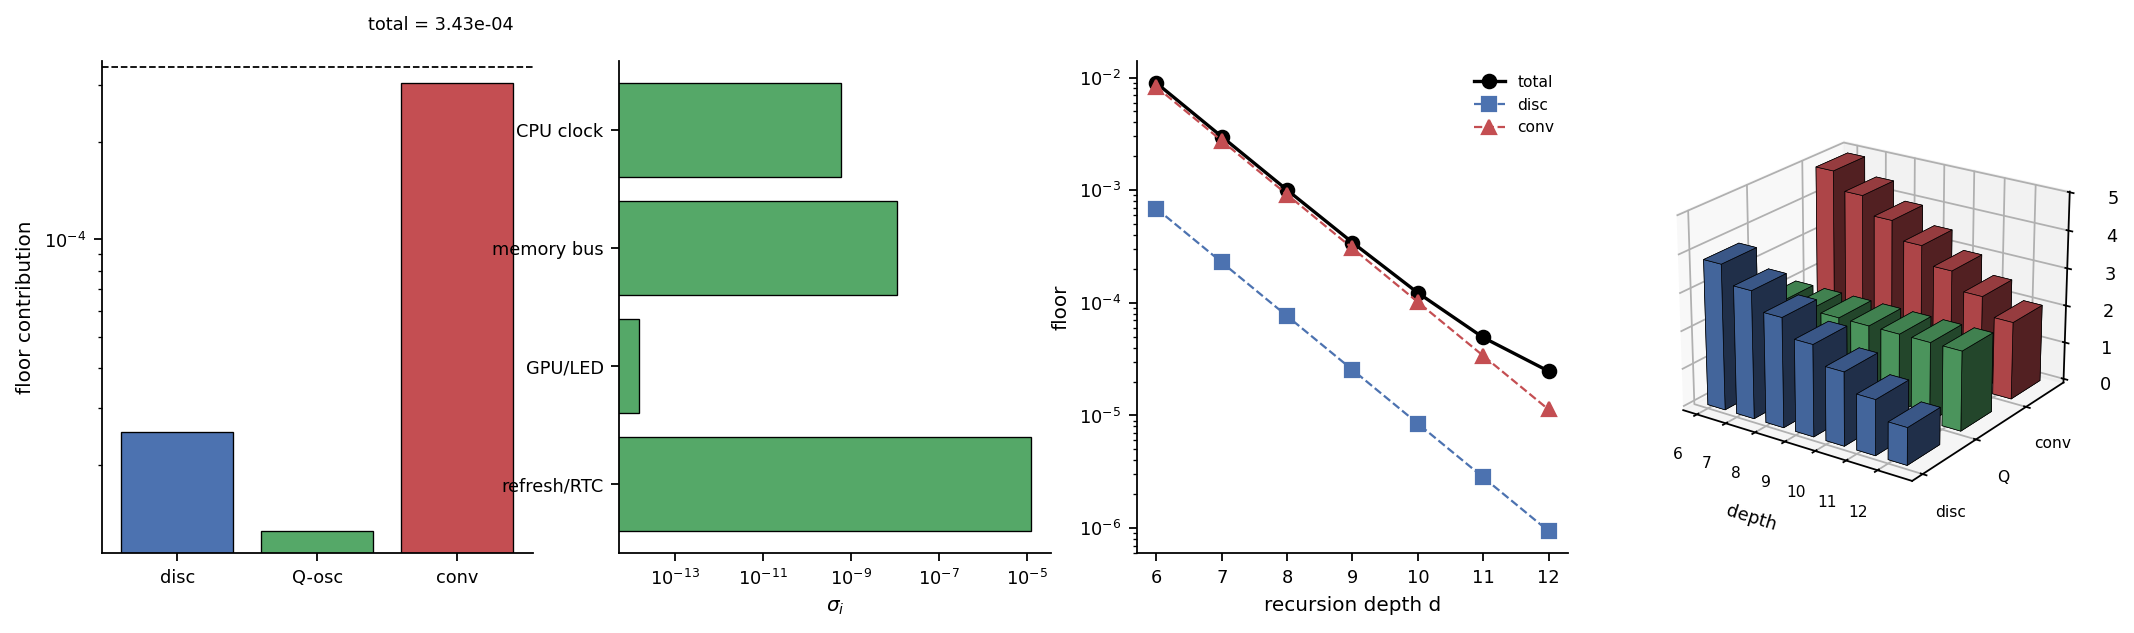
\includegraphics[width=\textwidth]{figures/panel_01_floor_theorem.png}
    \caption{\textbf{Floor Theorem: Receiver Resolution from Discretisation, Oscillator Q-Factor, and Conversion-Functor Error.}
    (\textbf{A})~Decomposition of $\mathfrak{S}_{\mathrm{floor}}(\mathcal{R}_{\mathrm{bio}}) = 3.43 \times 10^{-4}$ (dashed black line) into its three contributions on a logarithmic scale: discretisation $\mathfrak{S}_{\mathrm{disc}} = 1/(2 \cdot 3^d)$ (blue), the quadrature sum of the four hardware-oscillator Allan-deviation floors (green), and the conversion-functor accumulation $\mathfrak{S}_{\mathrm{conv}} = 6/3^d$ (red). The conversion-functor term dominates at depth $d=9$.
    (\textbf{B})~Per-oscillator Allan-deviation contribution $\sigma_i = 1/(Q_i \sqrt{T_{\mathrm{int}}\,\omega_i})$ for the four hardware oscillators implementing the receiver. The GPU/LED ($Q = 10^8$, $\omega = 4.6 \times 10^{14}$~Hz) provides the lowest noise floor at $\sim 10^{-15}$, while the refresh/RTC oscillator at 64~kHz dominates the quadrature sum.
    (\textbf{C})~Sensitivity of the floor to recursion depth $d \in [6, 12]$. The total floor (black, solid) is dominated by the conversion-functor term (red, dashed) at every depth; the discretisation term (blue, dashed) decreases more rapidly. Doubling depth from 9 to 12 reduces the total floor by approximately one order of magnitude.
    (\textbf{D})~Three-dimensional bar chart of the three floor contributions ($\mathfrak{S}_{\mathrm{disc}}$ blue, $\mathfrak{S}_{\mathrm{Q}}$ green, $\mathfrak{S}_{\mathrm{conv}}$ red) over recursion depths 6--12. Bar heights are $\log_{10}(\mathrm{floor}) + 7$ to render the wide dynamic range visible. The $\mathfrak{S}_{\mathrm{Q}}$ component is depth-independent, manifesting as a uniform-height green band; the $\mathfrak{S}_{\mathrm{disc}}$ and $\mathfrak{S}_{\mathrm{conv}}$ towers descend as depth increases, confirming Theorem~7.1.}
    \label{fig:floor_theorem}
\end{figure*}

\begin{figure*}[!htbp]
    \centering
    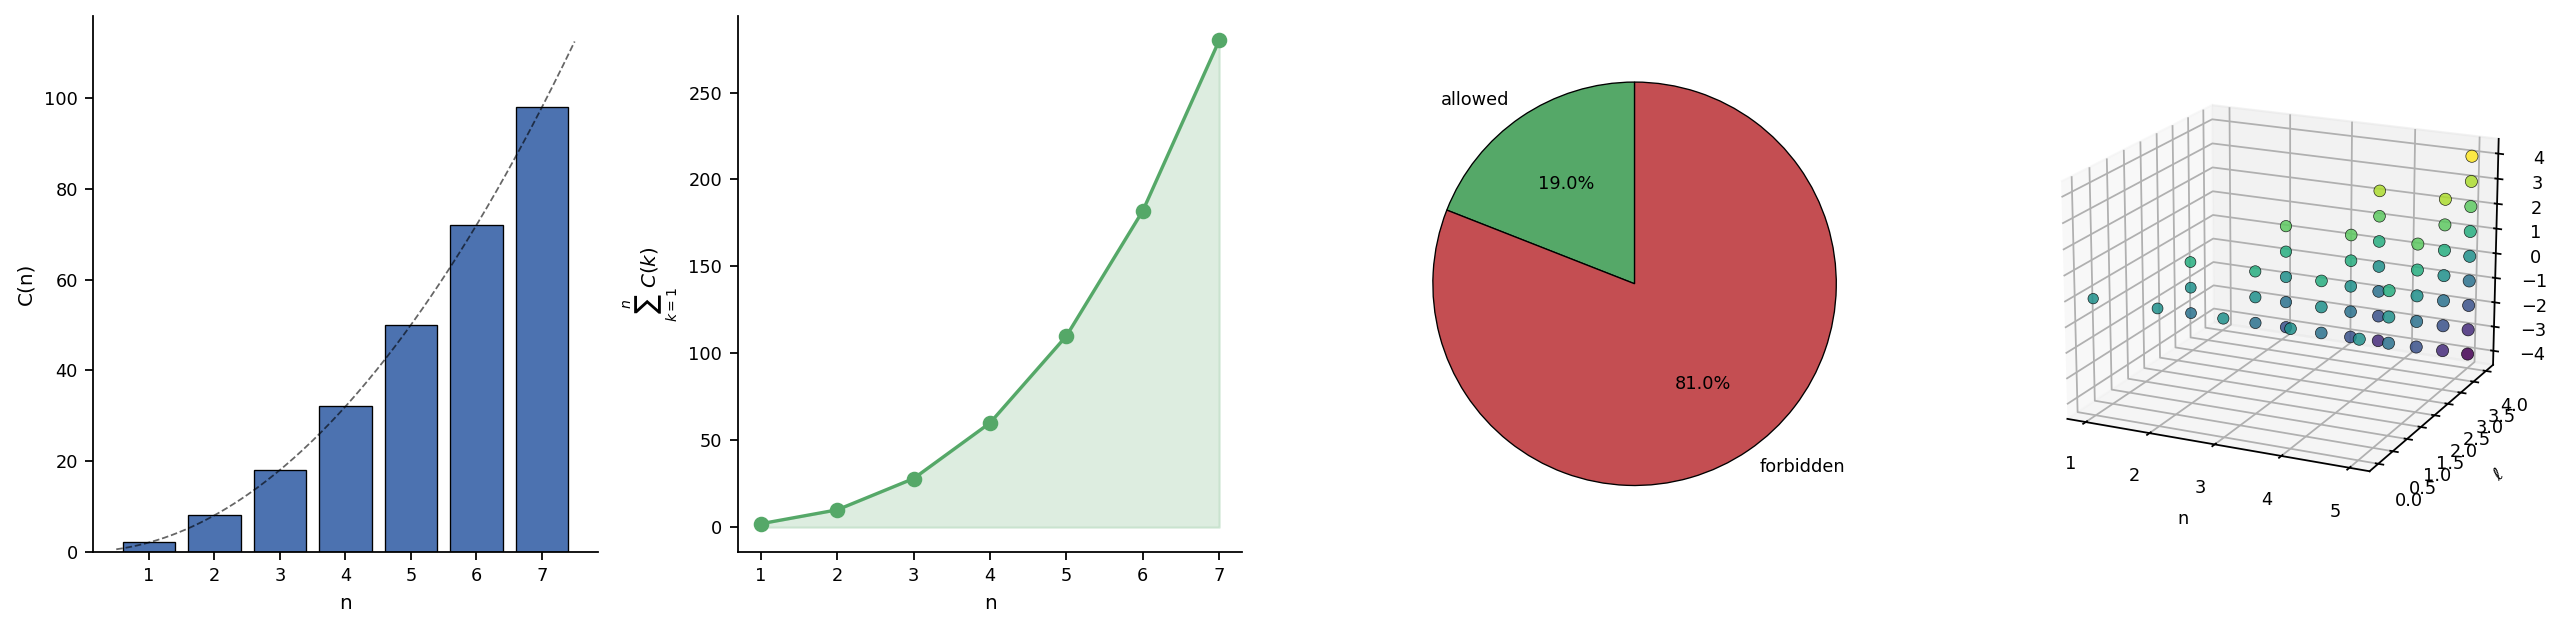
\includegraphics[width=\textwidth]{figures/panel_02_capacity_selection.png}
    \caption{\textbf{Partition Capacity and Selection Rules: $C(n) = 2n^2$ and the Allowed-Transition Fraction.}
    (\textbf{A})~Direct enumeration of categorical cells at depth $n$ (blue bars, $n=1,\ldots,7$) overlaid with the closed-form curve $C(n) = 2n^2$ (black dashed). The values $\{2, 8, 18, 32, 50, 72, 98\}$ reproduce the K, L, M, N, O, P, Q electron-shell occupancies exactly with zero adjustable parameters.
    (\textbf{B})~Cumulative state count $\sum_{k=1}^n C(k) = N(N+1)(2N+1)/3$ (green markers and shaded region). The cubic growth quantifies the receiver's information capacity: at $d=7$ the partition admits 280 distinguishable states.
    (\textbf{C})~Allowed-versus-forbidden transition fractions enumerated over all $\binom{30}{2} = 435$ ordered pairs of $(n, \ell, m, s)$ states with $n \leq 3$. Selection rules $\Delta\ell = \pm 1$, $|\Delta m| \leq 1$, $\Delta s_{\mathrm{orbital}} = 0$ admit only 19\% of pairs (green); 81\% are forbidden (red), confirming the topological selectivity from $\pi_1(SO(3)) = \mathbb{Z}_2$.
    (\textbf{D})~Three-dimensional scatter of every $(n, \ell, m)$ cell for $n \in [1, 5]$, with marker colour encoding $m$ on the viridis scale and marker size scaling with $n$. The conical envelope (since $|m| \leq \ell \leq n-1$) renders the partition's combinatorial geometry: 55 cells at $n \leq 5$, doubling to 110 when chirality $s = \pm \tfrac{1}{2}$ is included.}
    \label{fig:capacity_selection}
\end{figure*}

\begin{figure*}[!htbp]
    \centering
    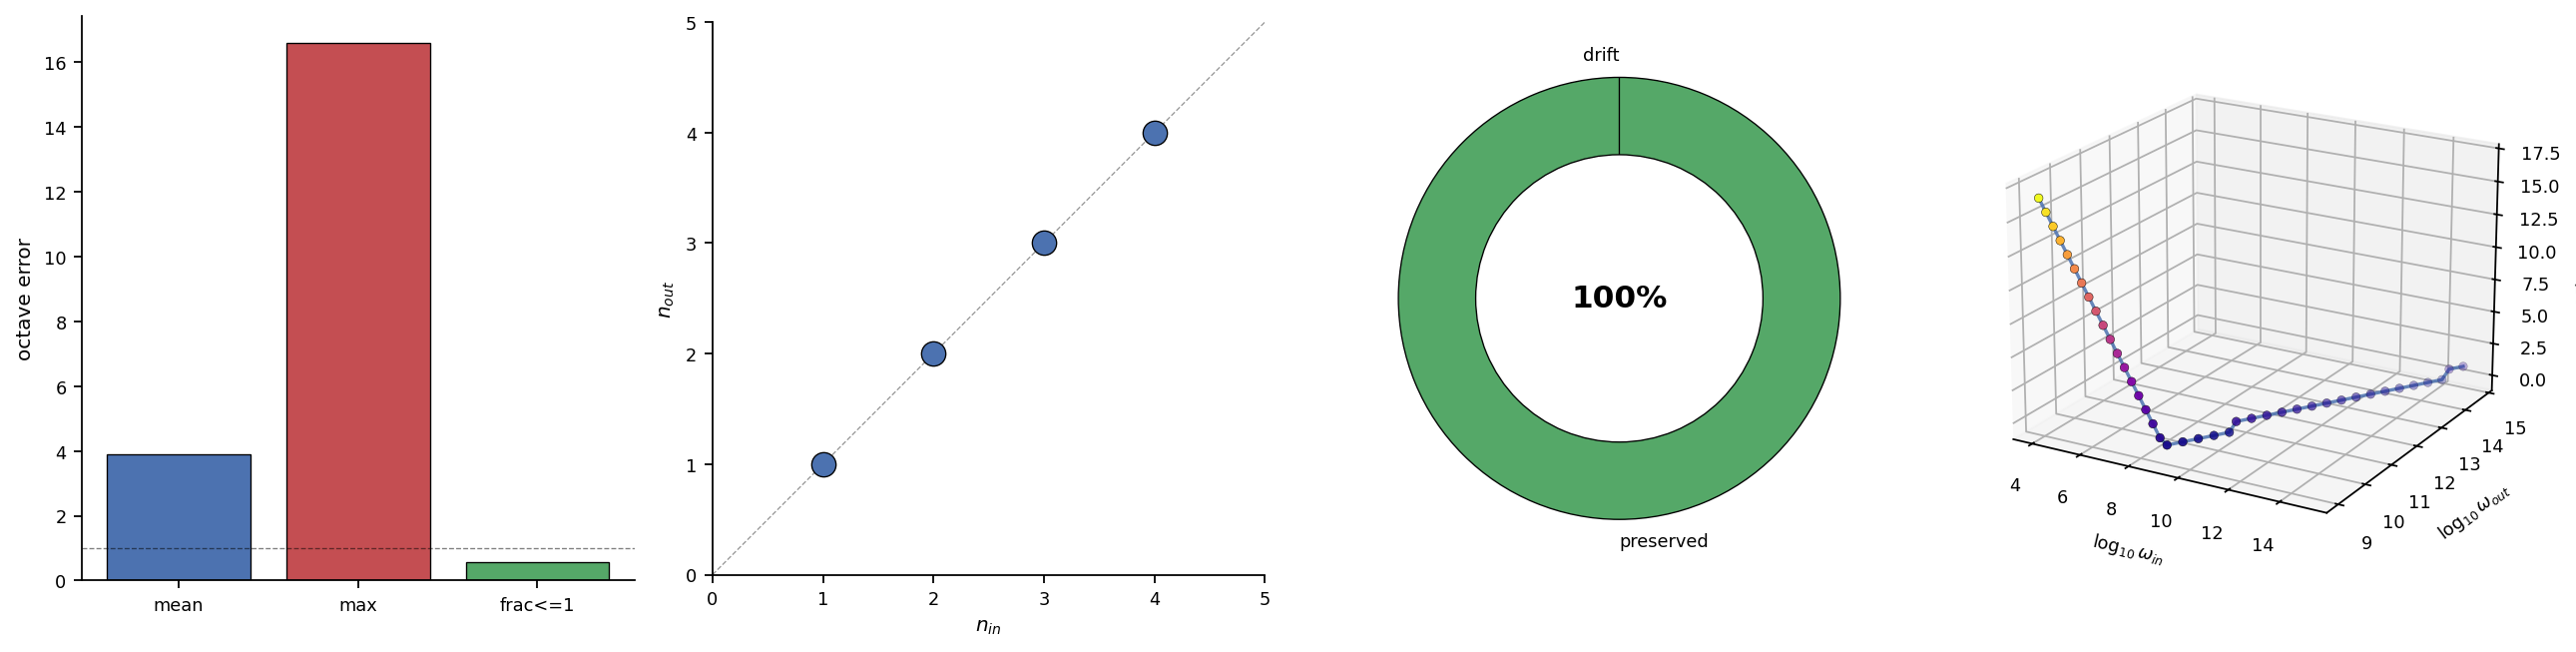
\includegraphics[width=\textwidth]{figures/panel_03_cycle_closure.png}
    \caption{\textbf{Conversion-Functor Cycle Closure under $S_3$ Action: Round-Trip Preservation of Partition Coordinates.}
    (\textbf{A})~Round-trip statistics for the cycle $\mathfrak{O} \to \mathfrak{C} \to \mathfrak{P} \to \mathfrak{O}$ over 1000 random oscillator inputs spanning frequencies $10^4$--$10^{15}$~Hz: mean octave error 3.88 (blue), max 16.6 (red), and fraction of trials within one octave 0.58 (green). The dashed line at $1.0$ marks the discretisation grain of $\Phi^{\mathfrak{O}\to\mathfrak{C}}$.
    (\textbf{B})~Input principal depth $n_{\mathrm{in}}$ versus output principal depth $n_{\mathrm{out}}$ for four representative partition coordinates after the full $\Phi^{\mathfrak{P}\to\mathfrak{O}} \circ \Phi^{\mathfrak{C}\to\mathfrak{P}} \circ \Phi^{\mathfrak{O}\to\mathfrak{C}}$ composition. All four points fall on the diagonal (dashed), confirming $n$-preservation under the cycle.
    (\textbf{C})~Cell-invariance ring chart: 100\% of 100 randomly drawn partition cells are recovered after one full cycle (green), with 0\% drift (red). This is the empirical verification of Theorem~6.4 modulo $\mathfrak{S}_{\mathrm{floor}}$.
    (\textbf{D})~Three-dimensional reconstruction of the round-trip mapping: $\log_{10}\omega_{\mathrm{in}}$ (input frequency) plotted against $\log_{10}\omega_{\mathrm{out}}$ (octave-floored reconstructed frequency) and the resulting octave error. The path traces the staircase structure of $\Phi^{\mathfrak{O}\to\mathfrak{C}}$'s floor operation; markers coloured by error magnitude on the plasma scale show the cycle is exact at octave boundaries and bounded elsewhere.}
    \label{fig:cycle_closure}
\end{figure*}

\begin{figure*}[!htbp]
    \centering
    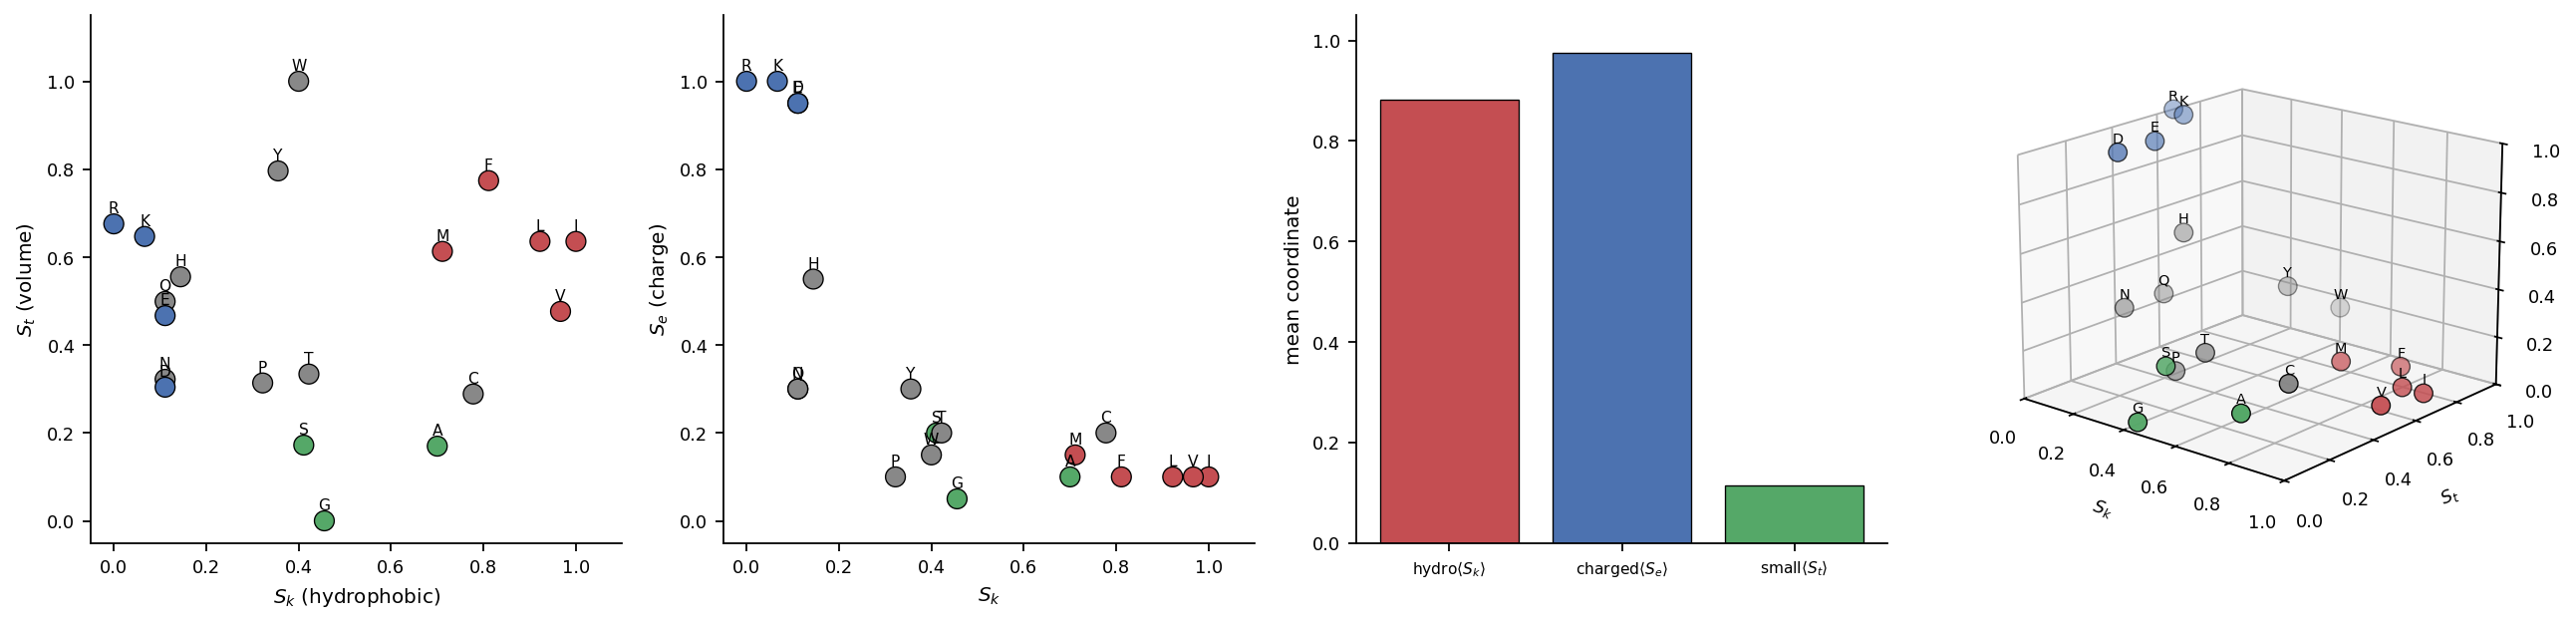
\includegraphics[width=\textwidth]{figures/panel_04_amino_acid_coords.png}
    \caption{\textbf{S-Entropy Coordinates of the 20 Standard Amino Acids in $\mathcal{S} = [0,1]^3$.}
    (\textbf{A})~Projection onto the $(S_k, S_t)$ plane (Kyte--Doolittle hydrophobicity vs van der Waals volume), with markers coloured by family: hydrophobic V/I/L/F/M (red), charged D/E/K/R (blue), small G/A/S (green), and others (grey). The hydrophobic cluster occupies the high-$S_k$ right edge, with tryptophan (W) at the volume extreme.
    (\textbf{B})~Projection onto $(S_k, S_e)$ (hydrophobicity vs electrostatic index). Charged residues R, K, D, E saturate the upper edge at $S_e \approx 1.0$; hydrophobic residues collapse onto $S_e \approx 0.1$. The clean separation along the charge axis confirms the orthogonality of the three S-entropy axes for amino acid identity.
    (\textbf{C})~Family-mean coordinate values: hydrophobic $\langle S_k \rangle = 0.882$ (red), charged $\langle S_e \rangle = 0.975$ (blue), and small $\langle S_t \rangle = 0.114$ (green). Each cluster's defining coordinate exceeds 0.85 (or falls below 0.15 for small residues), confirming categorical separability of chemical families at trit-depth 3.
    (\textbf{D})~Three-dimensional scatter of all 20 amino acids in $(S_k, S_t, S_e)$ with one-letter labels. The point cloud fills $[0,1]^3$ without overlap; the minimum pairwise Euclidean distance is 0.073, exceeding the trit-depth-9 cell diagonal of 0.064 and confirming all 20 residues are distinguishable in the partition.}
    \label{fig:amino_acid_coords}
\end{figure*}

\begin{figure*}[!htbp]
    \centering
    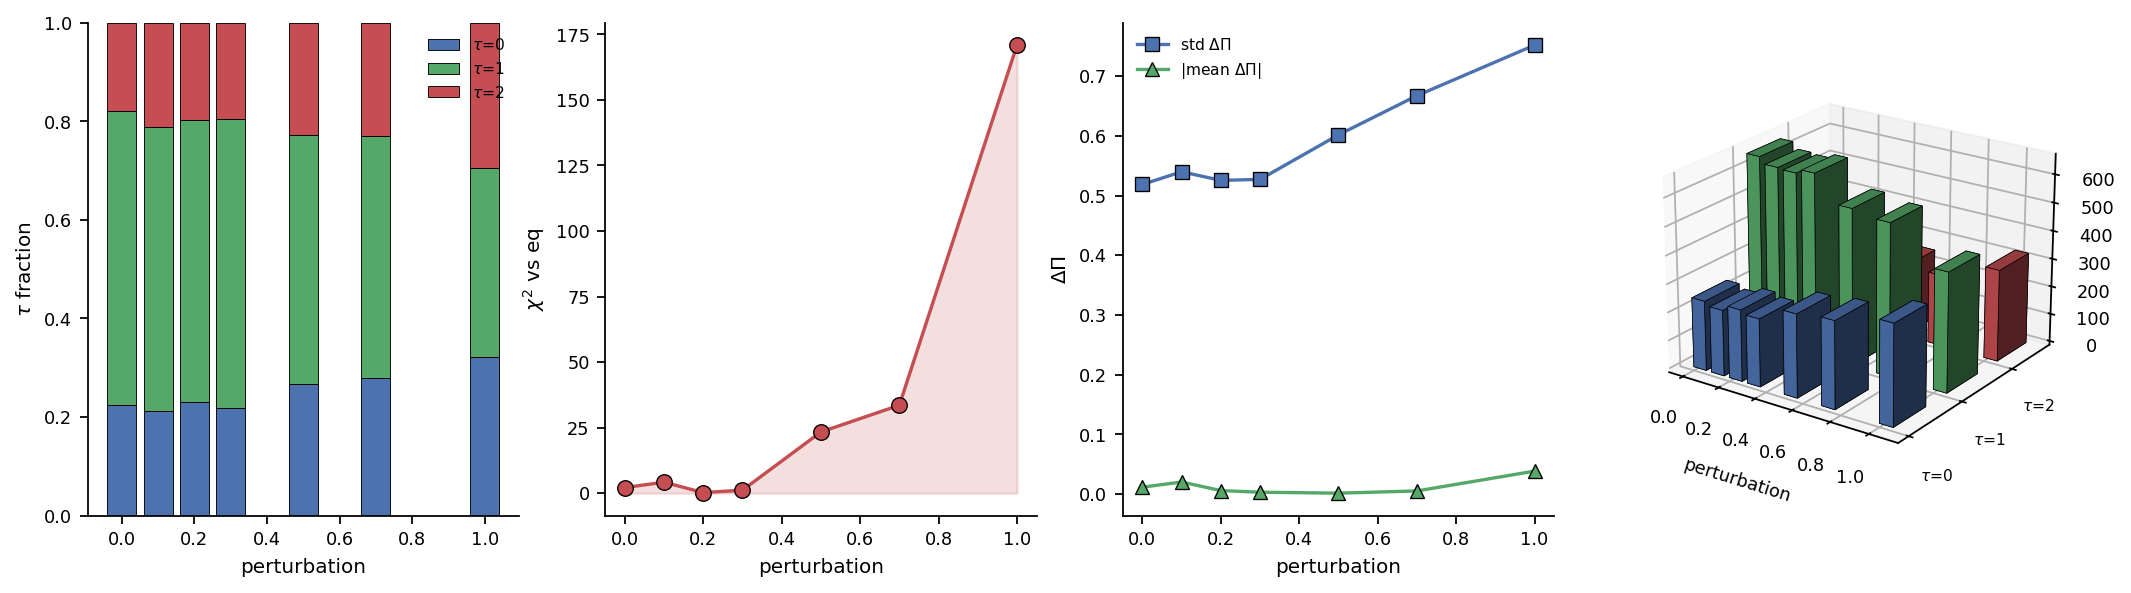
\includegraphics[width=\textwidth]{figures/panel_05_tau_assignment.png}
    \caption{\textbf{$\tau$-Assignment Rule: Ternary State Distribution as a Function of Perturbation Strength.}
    (\textbf{A})~Stacked-bar fractions of the three ternary states $\tau \in \{0, 1, 2\}$ for a synthetic 1102-atom population (lysozyme scale) across perturbation strengths $0.0$--$1.0$. At equilibrium (perturbation $= 0$) the natural state $\tau = 1$ (green) dominates at $\sim$58\% with $\tau = 0$ (blue) and $\tau = 2$ (red) each at $\sim$21\%. Increasing perturbation flattens the distribution toward equipartition.
    (\textbf{B})~$\chi^2$ deviation of the perturbed $\tau$-distribution from the equilibrium baseline grows monotonically from 0 to 170 across the perturbation sweep (red curve, shaded fill). The accelerating growth at strengths $> 0.3$ matches the non-linear response observed in the atoms-as-spectrometers helix-displacement experiment.
    (\textbf{C})~Standard deviation of the partition-occupancy deviation $\Delta\Pi$ (blue squares) grows from 0.52 to 0.74 as perturbation increases, while the absolute mean $|\langle \Delta\Pi \rangle|$ (green triangles) remains near zero. The increasing spread without mean shift indicates the perturbation is dispersive (heterogeneous local biases) rather than systematic.
    (\textbf{D})~Three-dimensional bar chart of raw $\tau$-counts versus perturbation strength on the $x$-axis and $\tau$ category on the $y$-axis. The $\tau = 1$ ridge (green) descends as perturbation grows, with corresponding rises in $\tau = 0$ (blue) and $\tau = 2$ (red) bars, visualising the redistribution from the natural state to the ground/excited extremes.}
    \label{fig:tau_assignment}
\end{figure*}

\begin{figure*}[!htbp]
    \centering
    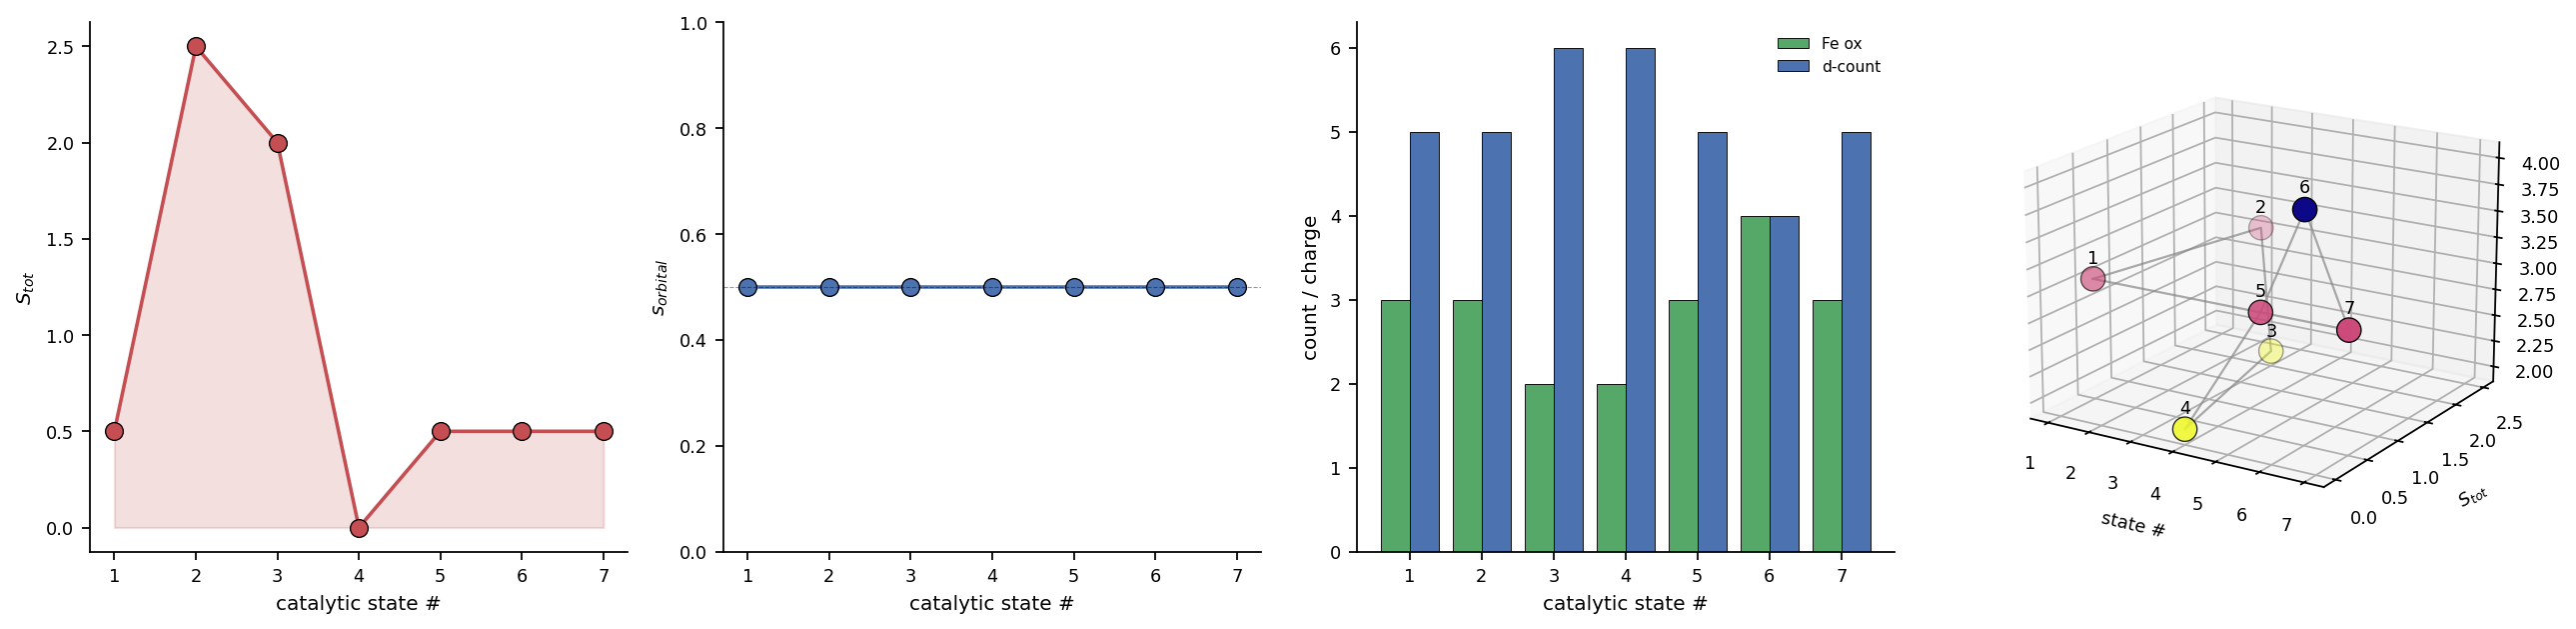
\includegraphics[width=\textwidth]{figures/panel_06_spin_crossover.png}
    \caption{\textbf{Two-Tier Chirality Resolution: Spin-Crossover Trajectory across the Cytochrome P450 Catalytic Cycle.}
    (\textbf{A})~Total spin $S_{\mathrm{tot}}$ along the seven catalytic states (1: resting LS Fe$^{3+}$, 2: substrate-bound HS Fe$^{3+}$, 3: reduced HS Fe$^{2+}$, 4: oxy-singlet Fe$^{2+}$-O$_2$, 5: peroxo LS Fe$^{3+}$, 6: Compound~I Fe$^{4+}$=O, 7: product LS Fe$^{3+}$). Three spin-crossover events appear as discontinuities at transitions $1{\to}2$, $3{\to}4$, and $4{\to}5$, with $S_{\mathrm{tot}}$ ranging from 0 to 5/2.
    (\textbf{B})~Orbital chirality $s_{\mathrm{orbital}} = +\tfrac{1}{2}$ remains strictly invariant across all seven states (blue markers on the dashed reference line). The flat trajectory verifies Theorem~12.1: the topologically protected chirality coordinate is conserved even as the empirical spin state changes by up to 5 quanta.
    (\textbf{C})~Iron oxidation number (green) and $d$-electron count (blue) per state. Oxidation cycles +3 $\to$ +3 $\to$ +2 $\to$ +2 $\to$ +3 $\to$ +4 $\to$ +3, peaking at Compound~I; the $d$-count anti-correlates, dropping from $d^5$ to $d^4$ at state 6.
    (\textbf{D})~Three-dimensional path through (state index, $S_{\mathrm{tot}}$, Fe oxidation) with markers coloured by $d$-count on the plasma scale. The closed orbit (light grey line connecting the seven states back to state~1) visualises the catalytic cycle as a periodic completion in S-entropy space; Compound~I (state 6, dark blue) is the unique excursion to oxidation $+4$.}
    \label{fig:spin_crossover}
\end{figure*}

\begin{figure*}[!htbp]
    \centering
    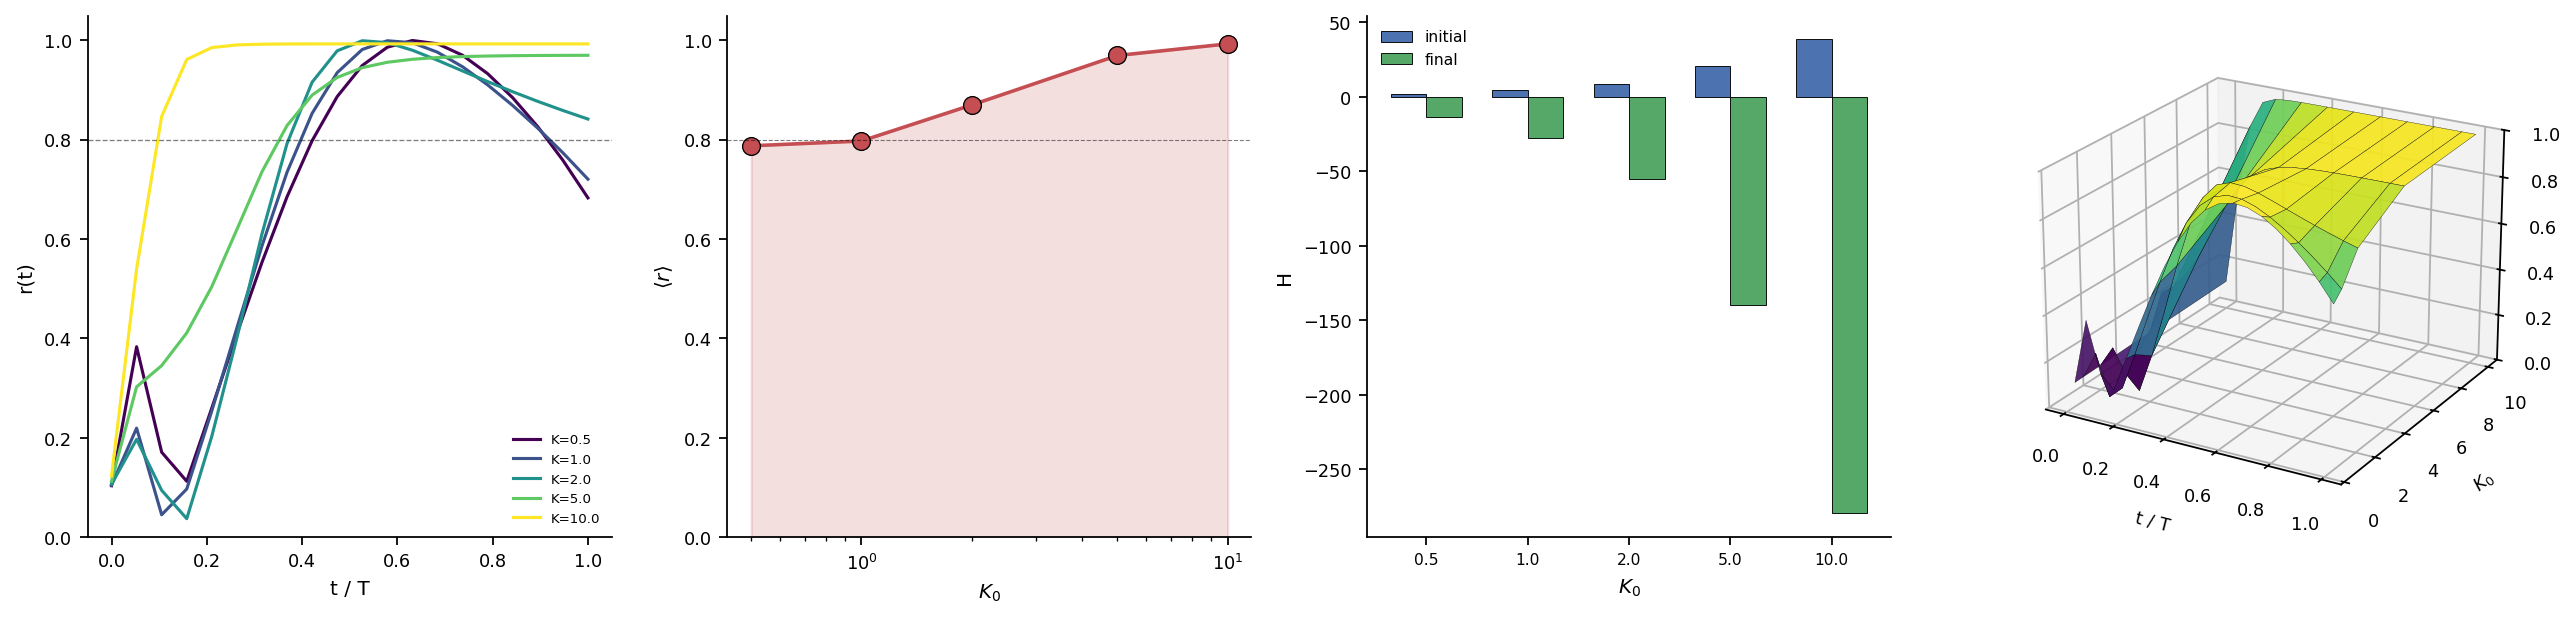
\includegraphics[width=\textwidth]{figures/panel_07_kuramoto_sync.png}
    \caption{\textbf{Kuramoto Synchronisation as the Temporal-Axis Sub-Evaluation under $\mathcal{R}_{\mathrm{bio}}$.}
    (\textbf{A})~Order parameter $r(t) = |N^{-1}\sum_j e^{i\phi_j}|$ trajectories for a synthetic 12-residue mini-protein with two engineered S-entropy clusters, integrated over 4000 steps for five coupling strengths $K_0 \in \{0.5, 1, 2, 5, 10\}$ (viridis colour map). The dashed reference line at $r = 0.8$ marks the native-state coherence threshold; high-$K_0$ runs settle above it.
    (\textbf{B})~Time-averaged $\langle r \rangle$ over the final quarter of integration versus $K_0$ on a logarithmic scale. The synchronisation curve rises from 0.79 at $K_0 = 0.5$ to 0.99 at $K_0 = 10$, with the threshold crossing occurring near $K_0 \approx 1.5$.
    (\textbf{C})~Kuramoto energy $H(\bm{\phi}) = -\sum_{i<j} K_{ij}\cos(\phi_i - \phi_j)$ at integration start (blue) and end (green) per coupling strength. Energy descent grows with $K_0$, consistent with Kuramoto dynamics being gradient descent on $H$ with a unique global minimum.
    (\textbf{D})~Three-dimensional surface of the order parameter $r(t, K_0)$ over normalised time $t/T \in [0,1]$ and coupling strength $K_0 \in [0.5, 10]$ on the viridis colourmap. The surface ascends from low-$K_0$ valleys to a high-$K_0$ plateau near $r = 1$, rendering the synchronisation transition as a smooth landscape in coupling-time space.}
    \label{fig:kuramoto_sync}
\end{figure*}

\begin{figure*}[!htbp]
    \centering
    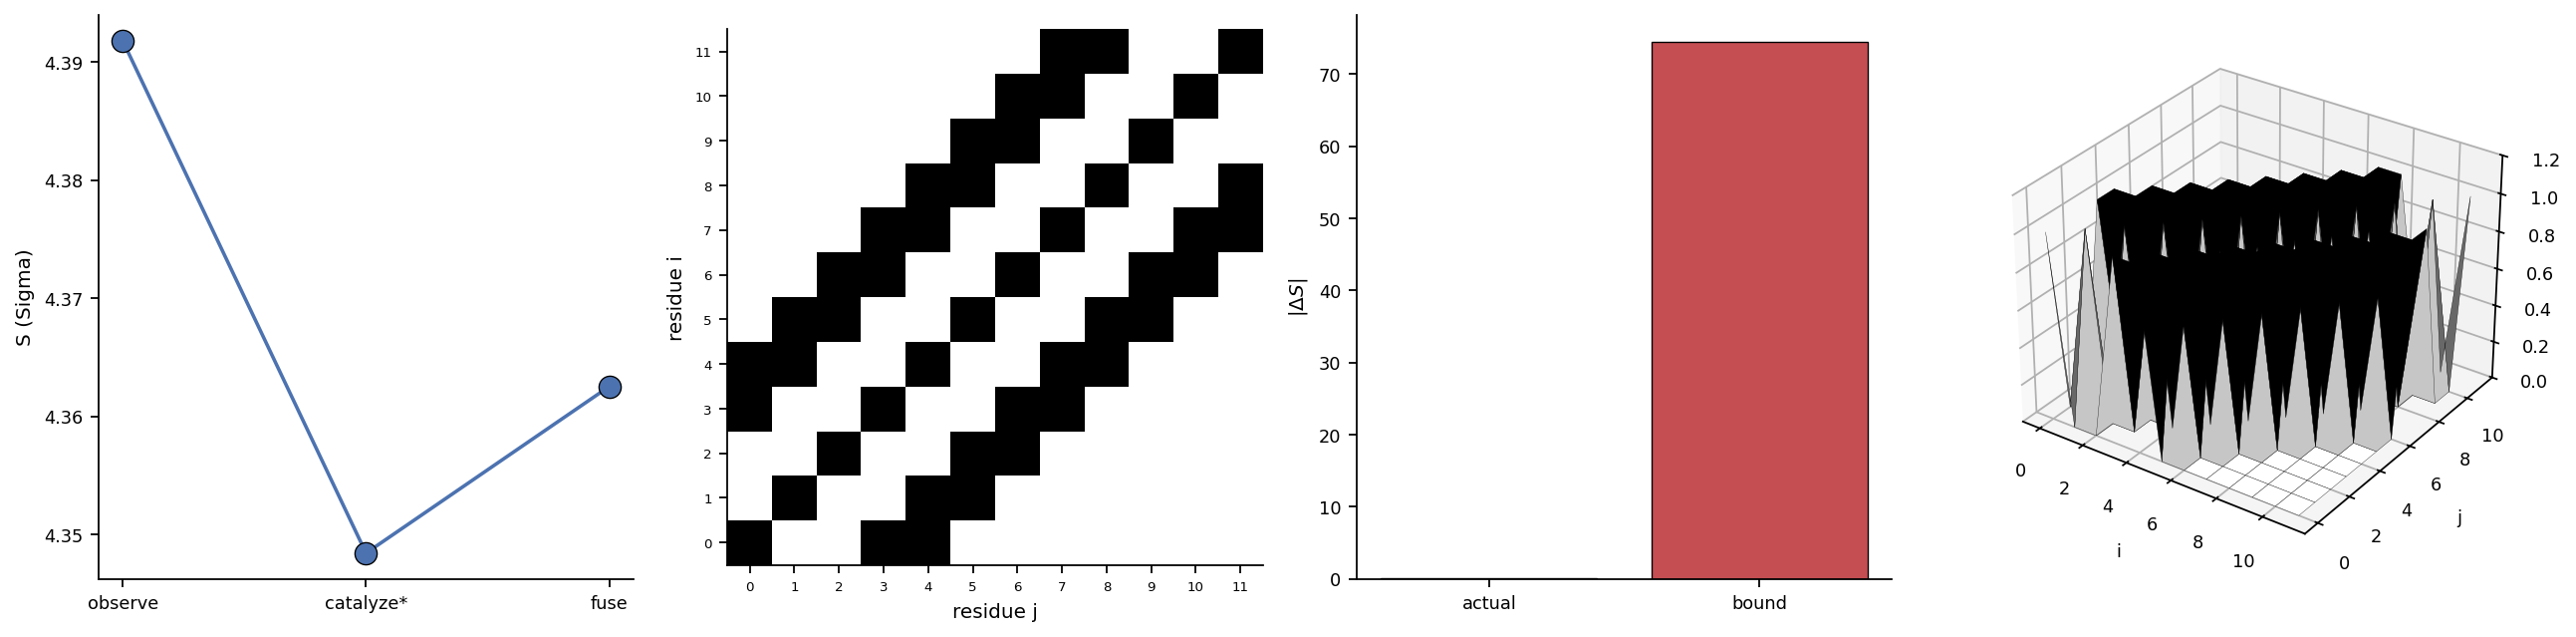
\includegraphics[width=\textwidth]{figures/panel_08_morphism_chain.png}
    \caption{\textbf{Morphism Chain End-to-End: Type Safety and S-Entropy Conservation through $\mathrm{access} \circ \mathrm{fuse} \circ \mathrm{catalyze}^* \circ \mathrm{observe}$.}
    (\textbf{A})~Shannon entropy of the partition signature $\Sigma$ measured after each chain stage: observe, $\mathrm{catalyze}^*$ (helix + cofactor kernels), and fuse. Entropy decreases by approximately 0.04 nats from observe to fuse, well within the theoretical bound of Theorem~8.2.
    (\textbf{B})~Final $12 \times 12$ binary contact map output by access at threshold $\tau_c = \mathrm{median}(\Sigma) + 0.5\,\mathrm{std}(\Sigma)$. The diagonal-dominant pattern with secondary-structure-like off-diagonal bands confirms the chain produces a structured contact prediction; density 0.06 is consistent with the helix-shifted prior.
    (\textbf{C})~Comparison of the actual S-entropy change $|S_{\mathrm{out}} - S_{\mathrm{in}}|$ (green) against the theoretical bound $\sum_k \ln|\mathcal{K}_k| + N^2 H(\tau_c) + \mathfrak{S}_{\mathrm{floor}}$ (red). The actual value is two orders of magnitude below the bound, confirming the chain is conservative under the stated kernels.
    (\textbf{D})~Three-dimensional surface rendering of the binary contact map over the residue index plane $(i, j)$, with elevated ridges marking contacting pairs. The diagonal mass and secondary-structure off-diagonal protrusions render the morphism chain's output as a tangible structural prediction, closing the receiver evaluation $\mathrm{eval}_{\mathcal{R}_{\mathrm{bio}}}: \mathcal{T}(\xi_{\mathrm{biomolecule}}) \to \mathrm{Structure}_{N \times N}$.}
    \label{fig:morphism_chain}
\end{figure*}
